% UI-as-Policy: capability-driven UI contracts for multi-tenant SaaS.
% Canonical full version for arXiv / technical report use.

\documentclass[11pt, reqno]{amsart}

% Page and typography.
\usepackage[margin=1in]{geometry}
\usepackage{microtype}
\usepackage[T1]{fontenc}
\usepackage[utf8]{inputenc}
\usepackage{lmodern}
\usepackage{enumitem}
\usepackage{amsfonts, amssymb}
\usepackage{booktabs}
\usepackage{tabularx}
\usepackage{array}
\usepackage{float}
\usepackage{needspace}
\usepackage{xcolor}
\usepackage{graphicx}
\usepackage{caption}
\usepackage{listings}
\usepackage{tikz}
\usepackage{url}
\usepackage[hidelinks]{hyperref}
\usetikzlibrary{arrows.meta, positioning, shapes.multipart, fit, calc, backgrounds, decorations.pathmorphing, decorations.pathreplacing}

\setlength{\emergencystretch}{2em}
\setlist[itemize]{leftmargin=1.6em, itemsep=0.25em, topsep=0.35em}
\setlist[enumerate]{leftmargin=1.8em, itemsep=0.25em, topsep=0.35em}

% Colors and listings.
\definecolor{CausifyBg}{RGB}{248,248,248}
\definecolor{CausifyFrame}{RGB}{220,220,220}
\definecolor{CausifyComment}{RGB}{110,110,110}
\definecolor{CausifyKeyword}{RGB}{36,74,140}
\definecolor{CausifyString}{RGB}{24,110,90}
\definecolor{CausifyNumber}{RGB}{125,125,125}

\lstdefinestyle{causify}{
  basicstyle=\ttfamily\footnotesize,
  backgroundcolor=\color{CausifyBg},
  frame=single,
  rulecolor=\color{CausifyFrame},
  framerule=0.4pt,
  framesep=6pt,
  xleftmargin=2pt,
  xrightmargin=2pt,
  numbers=left,
  numberstyle=\tiny\color{CausifyNumber},
  numbersep=8pt,
  keywordstyle=\bfseries\color{CausifyKeyword},
  commentstyle=\itshape\color{CausifyComment},
  stringstyle=\color{CausifyString},
  showstringspaces=false,
  breaklines=true,
  breakatwhitespace=true,
  postbreak=\mbox{\textcolor{CausifyNumber}{$\hookrightarrow$}\space},
  tabsize=2,
  columns=fullflexible,
  keepspaces=true,
  captionpos=b,
  aboveskip=0.8\baselineskip,
  belowskip=0.8\baselineskip
}

\lstdefinestyle{json}{
  style=causify,
  numbers=left,
  morestring=[b]",
  literate={\\_}{{\_}}1
}

\lstdefinestyle{typescript}{
  style=causify,
  morekeywords={const,let,var,export,import,from,return,interface,type,extends,async,await,if,else,for,while,break,switch,case,default,try,catch,throw,new,typeof,instanceof,Promise,true,false,null,undefined}
}

% Macros.
\newcommand{\system}{\textsc{Causify Platform}}
\newcommand{\console}{\textsc{Causify Console}}
\newcommand{\uiData}{UI-as-Data}
\newcommand{\uiPolicy}{UI-as-Policy}
\newcommand{\viewas}{\texttt{view\_as}}
\newcommand{\code}[1]{\texttt{\detokenize{#1}}}
\newcommand{\cmark}{\textcolor{green!60!black}{\ensuremath{\checkmark}}}
\newcommand{\xmark}{\textcolor{red!70!black}{\ensuremath{\times}}}

\newenvironment{authorbio}[1]{%
  \par\noindent\textbf{#1}\nobreakspace\ignorespaces
}{\par\vspace{0.4em}}

\title[UI-as-Policy]{The Sidebar Is a Security Boundary\\
\large UI-as-Policy: Unified Permission and Layout System for Multi-Tenant Platforms}

\author[Ghasemnezhad et al.]{Shayan Ghasemnezhad, Giacinto Paolo (GP) Saggese, Paul Smith, Heanh Sok, and Vedanshubhai Joshi}
\date{July 2026}

\begin{document}

\begin{abstract}
Multi-tenant SaaS products often develop a small, expensive lie. The backend knows what a user may do; the frontend guesses what the user should see. Those guesses drift as tenants, roles, and modules change. The result is familiar to anyone who has operated a real platform: buttons that end in HTTP 403, pages that load and then deny access, support tickets that trace back to stale conditionals, and a product surface that quietly stops matching the authorization model.

We present \uiPolicy{}, a production-tested pattern that treats the UI as a first-class policy surface. The backend materializes a tenant- and role-scoped UI contract at runtime. The web tier derives navigation, module visibility, layout, and client-side ability rules from that contract, while backend APIs continue to enforce authorization independently. Policy lives as data, so tenant onboarding and module changes become reviewed configuration updates rather than redeploys.

The paper contributes a name for the failure mode, a Truthful UX invariant for policy-gated surfaces, and an implementation pattern built around \uiData{}, server-built CASL abilities, and auditable support impersonation. We report production measurements from \system{}: seven modules defined in the policy store, 25+ permission subjects, 150+ layout fields, zero-deployment tenant onboarding, 73--100\% policy coverage on high-value UI surfaces, a 91\% ETag cache-hit rate for identity revalidation, and 856 ms P50 full-materialization latency for the \code{/v2/me} control-plane contract.
\end{abstract}

\maketitle
\markboth{GHASEMNEZHAD ET AL.}{UI-AS-POLICY}

\noindent\textbf{Keywords.} multi-tenant SaaS; authorization; UI policy; server-driven UI; impersonation; authorization drift; policy-as-data

\setcounter{tocdepth}{1}
\tableofcontents

% ##############################################################################
\section{Introduction}
\label{sec:introduction}

A multi-tenant product makes promises. Every route, button, module, and sidebar entry says something to the user. It says: this belongs to you; this will work; this is part of your world.

Those promises are easy to break. The backend may enforce authorization correctly, while the frontend carries a separate permission model made from route guards, role checks, feature flags, and tenant-specific conditionals. The two models rarely fail in one dramatic incident. They drift one small decision at a time. A restricted tenant sees a billing module. A support engineer clicks into a page that was never enabled for that role. A module fetches configuration, discovers the user cannot use it, and renders a blank shell.

That is not only ugly product behavior. It is authorization drift. The UI is now describing a world the backend will not honor.

We adopt a blunt rule.

\begin{quote}
\textbf{If the UI can lie about access, it is part of the security boundary.}
\end{quote}

\uiPolicy{} is the discipline we use to make that boundary honest. The backend remains the enforcement point. The UI does not become trusted security code. Instead, the UI is rendered from a server-materialized contract that comes from the same policy inputs used for authorization. The frontend stops guessing.

The core primitive is \uiData{}: a tenant- and role-scoped UI contract containing enabled modules, layout fragments, and the effective support context. The web tier consumes that contract to compose navigation and module layouts. It also builds the client-side ability model from a server-side profile, then exports packed rules for user-experience decisions. Backend APIs continue to authorize every request.

\paragraph{Concrete failure.}
During onboarding for a restricted tenant, a frontend conditional for a billing module was not updated with the backend entitlement record. The sidebar showed the billing link. The backend returned HTTP 403. Three support escalations later, the discrepancy traced back to a stale if-block. Under \uiPolicy{}, the sidebar is rendered from the server-materialized module list; there is no standalone billing conditional to forget.

\paragraph{Contributions.}
This paper makes four contributions.

\begin{itemize}
  \item It names the representation gap between backend enforcement and frontend rendering, then states a Truthful UX invariant for policy-gated surfaces.
  \item It describes \uiData{}, a production pattern where tenant modules and layout fragments are materialized as a runtime UI contract instead of being scattered through frontend code.
  \item It shows how server-built CASL abilities, module layout checks, and backend enforcement keep the client useful without making it trusted.
  \item It presents a view-as support workflow with immutable actor attribution, server-enforced allow-lists, signed effective-context headers, and searchable audit logs.
\end{itemize}

The implementation uses Next.js, Cognito, AWS Lambda, DynamoDB, iron-session, and CASL \cite{aws_cognito_user_pools,aws_cognito_groups,aws_lambda,aws_dynamodb,iron_session,casl_docs}. The pattern itself is not tied to those choices.

% ##############################################################################
\section{Authorization Drift}
\label{sec:problem}

Most SaaS platforms start with a clean idea. The backend enforces access. The frontend checks enough state to avoid showing nonsense. That works while the product is small.

Then tenants diverge. One customer buys Grid, another buys Horizon, a demo tenant gets DataMap, and support engineers need temporary visibility into each of them. A few flags become a few route guards. A layout component grows tenant-specific branches. A module entry appears in one sidebar but not another. The backend remains the final authority, yet the UI has become a second policy system without the same discipline.

We call the gap between these two models the \emph{representation gap}. It is the distance between what the backend will permit and what the UI presents as available.

\subsection{Requirements}
\label{sec:requirements}

A multi-tenant UI policy system must satisfy five requirements.

\begin{description}[leftmargin=2.2em, style=nextline]
  \item[R1. No stale gates.] Policy-gated UI elements shown to a user must correspond to backend operations the system will actually permit for the user's current tenant and role.
  \item[R2. Configuration over redeploy.] Enabling a tenant or changing a module entitlement should be a reviewed data change, not a code release.
  \item[R3. Safe impersonation.] Support engineers need the tenant's perspective without shared credentials and without bypassing the authorization model.
  \item[R4. Defense in depth.] The UI must never be the only barrier. Backend APIs authorize requests even when a browser is tampered with.
  \item[R5. Support at scale.] Operators need scoped concurrent sessions and searchable audit trails, especially when several engineers are debugging different tenants at the same time.
\end{description}

Traditional RBAC handles a useful slice of this problem \cite{sandhu_rbac}. ABAC gives a richer model for attribute-derived decisions \cite{nist_abac}. Feature flags help with release control \cite{fowler_feature_toggles}. Policy engines such as OPA, Cedar, and OpenFGA centralize authorization decisions \cite{opa_docs,cedar_docs,aws_verified_permissions,openfga_docs}.

None of those choices automatically tells the frontend what world to render. They answer what is allowed. They do not prescribe how permission decisions become navigation, layout, module configuration, and support workflow. That missing layer is where \uiPolicy{} sits.

\begin{table}[H]
  \centering
  \small
  \begin{tabularx}{\textwidth}{X c c c}
    \toprule
    \textbf{Need} & \textbf{RBAC / ABAC} & \textbf{Feature flags} & \textbf{\uiPolicy{}} \\
    \midrule
    Backend authorization & \cmark & \xmark & \cmark \\
    Tenant-level variability & Partial & \cmark & \cmark \\
    UI derived from policy & \xmark & Partial & \cmark \\
    Config-only tenant changes & Partial & \cmark & \cmark \\
    Auditable view-as support & \xmark & \xmark & \cmark \\
    Defense against stale UI gates & \xmark & \xmark & \cmark \\
    \bottomrule
  \end{tabularx}
  \caption{Where \uiPolicy{} fits. It does not replace authorization frameworks. It uses their decisions to make the rendered interface truthful.}
  \label{tab:comparison}
\end{table}

\subsection{The Truthful UX invariant}
\label{sec:truthful_ux}

For policy-gated surfaces, we use the following invariant.

\begin{quote}
\textbf{A rendered UI affordance must be backed by a server-side policy decision in the same effective tenant and role context.}
\end{quote}

The invariant is intentionally narrow. It does not claim every pixel on the page is authorization-sensitive. A help link or account menu may be universal. It does claim that navigation, modules, layouts, and policy-gated actions should not be rendered from a parallel frontend guess.

% ##############################################################################
  \clearpage
  \section{System Overview}
  This section introduces the end-to-end flow and the artifacts exchanged
  between components. The key is that the backend produces a \emph{materialized}
  UI contract scoped by tenant and role, and the frontend renders it
  without inventing policy.

% ==============================================================================
  \subsection{High-level architecture}
  Figure~\ref{fig:architecture} shows the main components and control
  flow.

\begin{figure}[H]
  \centering
  \resizebox{\textwidth}{!}{%
  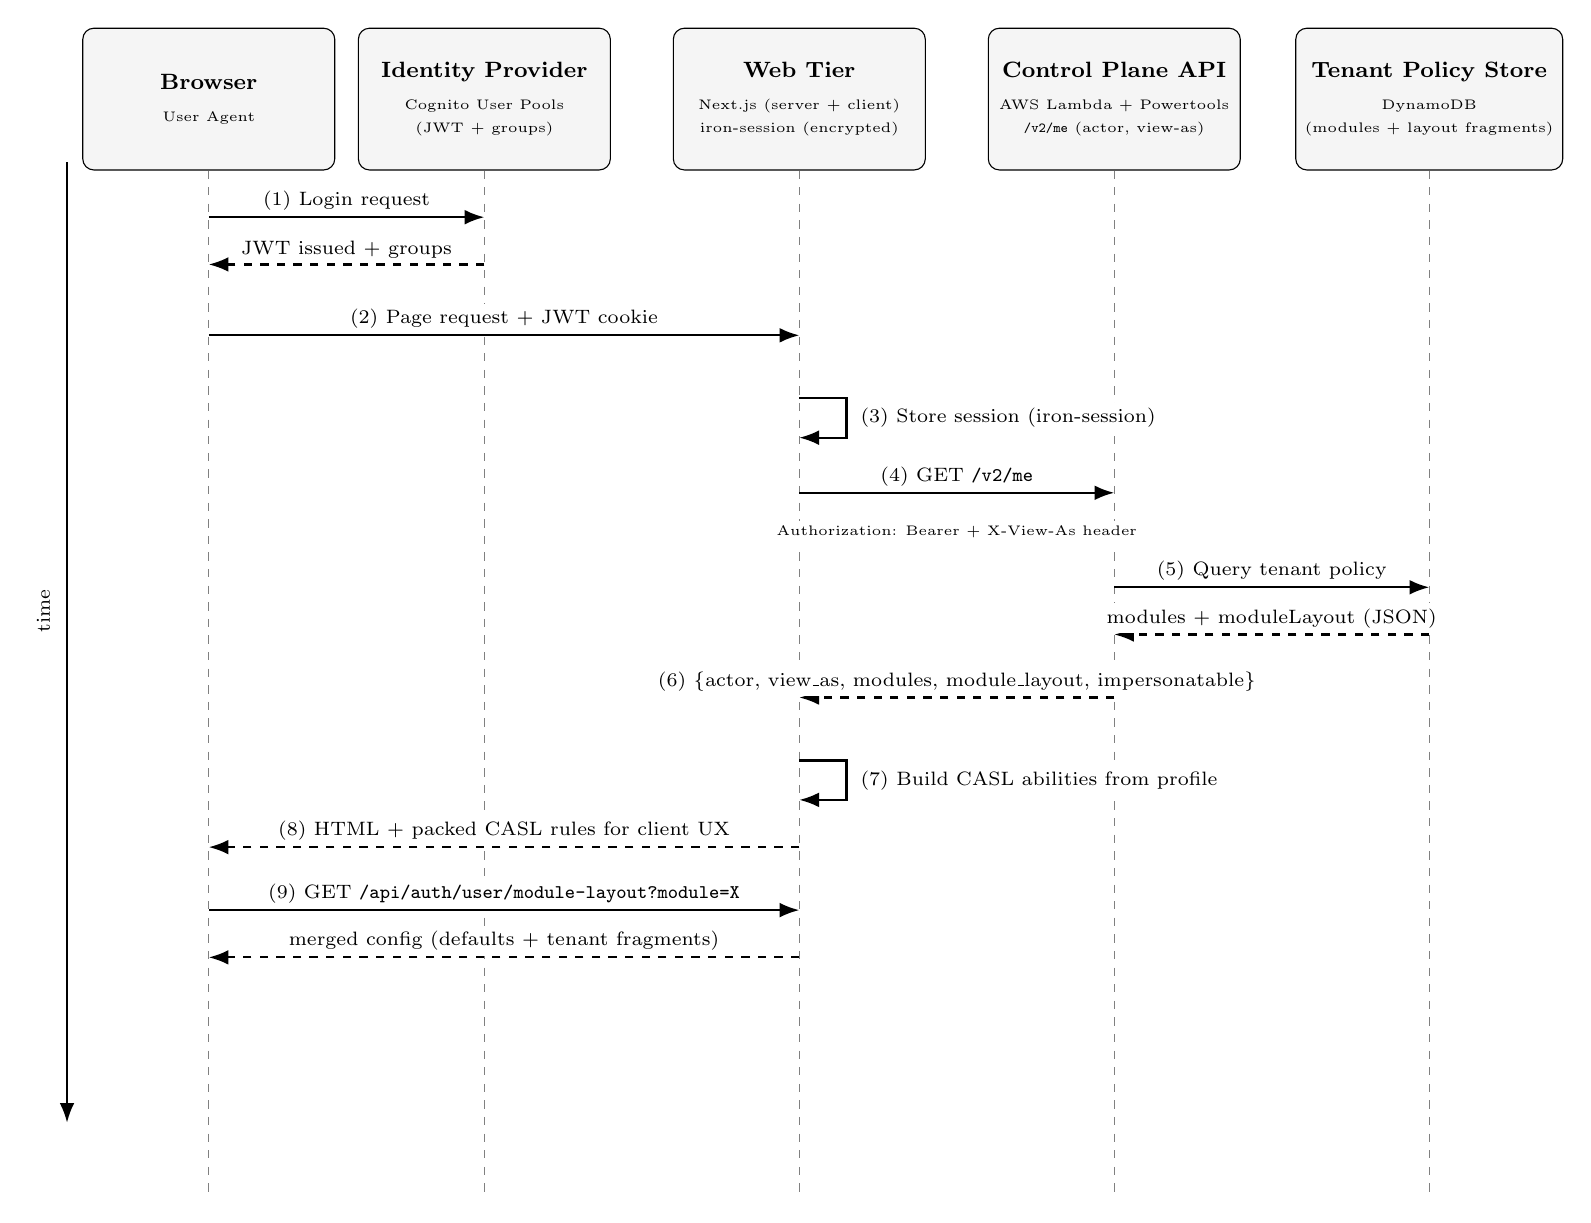
\begin{tikzpicture}[
    % Styles
    actor/.style={draw, rectangle, rounded corners, align=center, minimum width=32mm,
                  minimum height=18mm, font=\footnotesize, fill=gray!8},
    arrow/.style={-{Latex[length=2.5mm]}, thick},
    returnarrow/.style={-{Latex[length=2.5mm]}, thick, dashed},
    lbl/.style={font=\scriptsize, fill=white, inner sep=2pt, align=center},
    lifeline/.style={dashed, gray}
  ]
    % === Actor boxes (top) with full descriptions ===
    \node[actor] (user) at (0,0) {\textbf{Browser}\\[2pt]\tiny User Agent};

    \node[actor] (idp) at (3.5,0) {\textbf{Identity Provider}\\[2pt]\tiny Cognito User Pools\\[-1pt]\tiny (JWT + groups)};

    \node[actor] (web) at (7.5,0) {\textbf{Web Tier}\\[2pt]\tiny Next.js (server + client)\\[-1pt]\tiny iron-session (encrypted)};

    \node[actor] (api) at (11.5,0) {\textbf{Control Plane API}\\[2pt]\tiny AWS Lambda + Powertools\\[-1pt]\tiny \texttt{/v2/me} (actor, view-as)};

    \node[actor] (ddb) at (15.5,0) {\textbf{Tenant Policy Store}\\[2pt]\tiny DynamoDB\\[-1pt]\tiny (modules + layout fragments)};

    % === Lifelines ===
    \draw[lifeline] (user.south) -- ++(0,-13);
    \draw[lifeline] (idp.south) -- ++(0,-13);
    \draw[lifeline] (web.south) -- ++(0,-13);
    \draw[lifeline] (api.south) -- ++(0,-13);
    \draw[lifeline] (ddb.south) -- ++(0,-13);

    % === Messages ===

    % 1. Login to IdP
    \draw[arrow] (0,-1.5) -- node[lbl, above] {(1) Login request} (3.5,-1.5);
    \draw[returnarrow] (3.5,-2.1) -- node[lbl, above] {JWT issued + groups} (0,-2.1);

    % 2. Page request with JWT
    \draw[arrow] (0,-3) -- node[lbl, above] {(2) Page request + JWT cookie} (7.5,-3);

    % 3. Store session (self-call)
    \draw[arrow] (7.5,-3.8) -- ++(0.6,0) -- ++(0,-0.5) -- ++(-0.6,0);
    \node[lbl, right] at (8.2,-4.05) {(3) Store session (iron-session)};

    % 4. Fetch profile /v2/me
    \draw[arrow] (7.5,-5) -- node[lbl, above] {(4) GET \texttt{/v2/me}} (11.5,-5);
    \node[lbl] at (9.5,-5.5) {\tiny Authorization: Bearer + X-View-As header};

    % 5. Query tenant policy
    \draw[arrow] (11.5,-6.2) -- node[lbl, above] {(5) Query tenant policy} (15.5,-6.2);
    \draw[returnarrow] (15.5,-6.8) -- node[lbl, above] {modules + moduleLayout (JSON)} (11.5,-6.8);

    % 6. Return materialized UI contract
    \draw[returnarrow] (11.5,-7.6) -- node[lbl, above] {(6) \{actor, view\_as, modules, module\_layout, impersonatable\}} (7.5,-7.6);

    % 7. Build CASL abilities (self-call)
    \draw[arrow] (7.5,-8.4) -- ++(0.6,0) -- ++(0,-0.5) -- ++(-0.6,0);
    \node[lbl, right] at (8.2,-8.65) {(7) Build CASL abilities from profile};

    % 8. Return HTML + packed rules
    \draw[returnarrow] (7.5,-9.5) -- node[lbl, above] {(8) HTML + packed CASL rules for client UX} (0,-9.5);

    % 9. Lazy load module layout
    \draw[arrow] (0,-10.3) -- node[lbl, above] {(9) GET \texttt{/api/auth/user/module-layout?module=X}} (7.5,-10.3);
    \draw[returnarrow] (7.5,-10.9) -- node[lbl, above] {merged config (defaults + tenant fragments)} (0,-10.9);

    % Time arrow on left
    \draw[-{Latex[length=2.5mm]}, thick] (-1.8,-0.8) -- (-1.8,-13);
    \node[font=\scriptsize, rotate=90] at (-2.1,-6.5) {time};

  \end{tikzpicture}%
  }
  \caption{\system{} sequence diagram showing the complete request lifecycle.
  (1--2) Browser authenticates via Cognito and receives JWT with group claims.
  (3--4) Web Tier stores session and fetches materialized profile from Control Plane.
  (5--6) Control Plane queries DynamoDB for tenant policy and returns the UI contract.
  (7--8) Server builds CASL abilities and returns HTML with packed rules.
  (9) Module layouts are lazy-loaded on demand.}
  \label{fig:architecture}
\end{figure}

% ==============================================================================
  \subsection{Request lifecycle (what happens on a typical page load)}
  The core request lifecycle is:

  \begin{enumerate}
    \item \textbf{Authentication:} a user authenticates via Cognito and
      the web tier receives a JWT that includes group membership
      \cite{aws_cognito_user_pools,aws_cognito_groups}.

    \item \textbf{Control-plane materialization (\texttt{/v2/me}):} the
      web tier calls the control plane with \texttt{Authorization: Bearer
      \ldots} and optionally \texttt{X-View-As: tenant\_id=\ldots;role=\ldots}. The
      Lambda middleware validates the token, computes \texttt{user\_role},
      computes an \texttt{impersonatable} allow-list, validates \viewas{}
      selections against that allow-list, and returns:
      \begin{itemize}
        \item \texttt{actor}: immutable identity (who is calling),

        \item \texttt{view\_as}: effective tenant/role and derived modules/layout,

        \item \texttt{impersonatable}: permissible \viewas{} targets for
          support/QA.
      \end{itemize}
      The response includes caching and ETag support to reduce repeated materialization
      overhead (useful when the UI pings ``who am I?'' often).

    \item \textbf{Server-authoritative abilities:} the web tier builds
      the canonical permission model from the server-side session
      profile and exports packed rules for the client (CASL)
      \cite{casl_docs}. The client uses these rules for UX (what to show),
      while backend APIs remain authoritative for security (what is allowed).

    \item \textbf{Runtime UI composition:} the UI composes navigation
      and module defaults from \texttt{module\_layout} returned by \texttt{/v2/me}.
      Module-specific layout is lazily loaded and merged with shipped defaults,
      so configuration can be partial (override the sidebar, not the
      universe).
  \end{enumerate}

% ==============================================================================
  \subsection{Key abstractions and artifacts}
  Table~\ref{tab:artifacts} summarizes the artifacts that make the
  system composable and auditable.

  \begin{table}[H]
    \centering
    \small
    \begin{tabularx}{\textwidth}{>{\ttfamily\raggedright\arraybackslash}p{2.6cm} >{\raggedright\arraybackslash}p{2.8cm} X X}
      \toprule
      \textnormal{\textbf{Artifact}} & \textbf{Where defined} & \textbf{Produced by} & \textbf{Used for} \\
      \midrule
      actor & JWT + derived claims & \texttt{/v2/me} (Lambda) & Auditability: the real caller identity never changes. \\
      view\_as & \texttt{X-View-As} header & \texttt{/v2/me} (validated) & Effective tenant/role context for modules + layout. \\
      impersonatable & Derived from actor role & \texttt{/v2/me} & Guardrail: explicit allow-list of \viewas{} targets. \\
      modules & Tenant policy record & \texttt{/v2/me} & Capability list for UI composition and ability building. \\
      module\_layout & Tenant policy (JSON) & \texttt{/v2/me} & Structured UI contract: navigation + module defaults. \\
      \textnormal{Packed CASL rules} & Ability builder & \texttt{/api/\ldots/ability} & Client UX consistency: hide forbidden UI\@. \\
      \bottomrule
    \end{tabularx}
    \caption{The system's core artifacts: identity, effective context, capability
    set, and UI contract. The same policy inputs drive both authorization
    and UX.}
    \label{tab:artifacts}
  \end{table}

% ==============================================================================
  \subsection{Why this is different from ``dynamic UI''}
  Many systems have tenant-specific UIs. The distinguishing property
  here is not mere variability; it is \emph{policy alignment}.\@ \uiPolicy{}
  ensures that what the user sees is derived from the same tenant/role-scoped
  policy that determines what the system will allow. In short: the UI
  stops improvising.

% ==============================================================================
  \subsection{Module architecture: independence with shared policy}
  \label{sec:modules}

  \system{} implements a modular architecture where each functional area
  operates as an \emph{independent module}. Every module follows an identical
  structural pattern:

  \begin{itemize}
    \item \textbf{Server layout} (\texttt{layout.tsx}): enforces CASL access
      before rendering.
    \item \textbf{Client component} (\texttt{client.tsx}): interactive UI,
      state management, and data fetching.
    \item \textbf{Dedicated API routes} (\texttt{/api/\{module\}/}): inherit
      the same CASL and \viewas{} context.
  \end{itemize}

  This yields a key property: modules are \emph{independently evolvable} and
  can be enabled or disabled per tenant via policy without creating dead
  routes or broken doors. Listing~\ref{lst:module_layout} illustrates the protection pattern.

  \begin{samepage}
  \begin{lstlisting}[style=typescript,caption={Module protection pattern: server layout enforces CASL before rendering.},label={lst:module_layout}]
// app/(protected)/(app)/{module}/layout.tsx
import { requireAccess } from '@/lib/core/casl/server'

export default async function ModuleLayout({
  children
}: { children: React.ReactNode }) {
  await requireAccess('module-name')
  return <>{children}</>
}
\end{lstlisting}
  \end{samepage}

% ##############################################################################
\section{Policy Model}
\label{sec:policy_model}

The policy model has two layers. The first decides which modules exist for a tenant and role. The second decides which features and actions are available inside those modules.

\subsection{Modules and layout as data}
\label{sec:module_policy}

Module access is stored per tenant and role in DynamoDB. A policy record contains an enabled-module list and a \code{moduleLayout} object with structured UI fragments. The control plane reads this record during \code{/v2/me} materialization and merges tenant fragments with shipped defaults.

Tenant changes are therefore small and reviewable. Enabling DataMap for a pilot tenant or switching a sidebar mode is a data change. Adding a new module type still requires code, since a new module brings routes, components, handlers, and documentation. That is the right boundary: routine tenant variability belongs in data; new product surface belongs in code review.

Malformed configuration is rejected during materialization. Partial configuration is allowed only when it can be safely merged with defaults. A tenant can override one sidebar group without redefining the whole navigation model.

\subsection{Server-built abilities}
\label{sec:abilities}

Fine-grained permissions are expressed with CASL, an isomorphic JavaScript authorization library that serializes ability rules between server and client \cite{casl_docs}. In our deployment the ability model covers three actions, \code{view}, \code{manage}, and \code{use}, across 25+ subjects. Those subjects include modules, generic pages, feature permissions, sub-module subjects, and config-derived subjects such as \code{module:config:integration:enabled}.

The server builds the ability object from the materialized profile. The client receives packed rules and uses them only for UX decisions: hiding buttons, disabling menu entries, and suppressing unavailable panels. Backend APIs still enforce authorization independently. A browser that tampers with packed rules may fool itself; it does not gain backend access.

\subsection{No hidden second policy language}
\label{sec:no_second_policy}

The trap in many products is accidental policy language. A frontend branch like \code{if (tenant === "acme")} looks harmless. Ten of them become an undocumented entitlement system.

\uiPolicy{} draws a hard line. Frontend code may render from a contract. It may not invent access. The contract may be generated by RBAC, ABAC, a policy engine, a module registry, or a mix of those. What matters is that the rendered UI consumes the materialized decision instead of re-creating it.

\begin{table}[H]
  \centering
  \small
  \begin{tabularx}{\textwidth}{X r X}
    \toprule
    \textbf{Policy surface} & \textbf{Scale} & \textbf{Runtime effect} \\
    \midrule
    Modules in policy store & 7 & Drives navigation, dashboard cards, and module route access. \\
    CASL permission subjects & 25+ & Controls module, feature, page, sub-module, and config-derived access. \\
    \code{moduleLayout} fields & 150+ & Shapes sidebar mode, module defaults, settings tabs, feedback surfaces, and per-module fragments. \\
    Sidebar modes & 6 & Lets tenants vary navigation behavior without code forks. \\
    Tenant onboardings requiring deployment & 0 & Normal onboarding is a policy-store update plus identity assignment. \\
    \bottomrule
  \end{tabularx}
  \caption{Policy surface in the production deployment. Counts are taken from the deployed UI and control-plane configuration.}
  \label{tab:policy_surface}
\end{table}

% ##############################################################################
  \section{Runtime Composition: Making the UI Tell the Truth}
  This section describes how the web tier turns the UI contract into pixels
  without giving the browser a second job as an authorization engine.

% ==============================================================================
  \subsection{Abilities: one source of truth, exported for UX}
  Authorization is enforced server-side, but the UI still needs to know
  what to show. We use CASL \cite{casl_docs} to represent abilities and explicitly
  avoid duplicating rules in the frontend.

  \paragraph{Design.}
  \begin{itemize}
    \item The server builds the canonical ability from session-backed profile
      data (modules + role).

    \item The server serializes the ability rules using CASL's packed format.

    \item The client unpacks these rules to construct an identical ability
      object for UI/UX gating only.
  \end{itemize}

  \begin{samepage}
  \begin{lstlisting}[style=typescript,caption={Server-authoritative abilities: rules are built server-side and packed for client use. The backend remains the enforcement point.},label={lst:casl_pack}]
import { packRules } from '@casl/ability/extra'

// GET /api/auth/user/ability
const ability = await getUserAbility()
return { rules: packRules(ability.rules) }
\end{lstlisting}
  \end{samepage}

  \paragraph{Two-layer protection (by design).}
  The client uses the ability to hide inaccessible UI elements and prevent
  dead ends. Server components and API routes still enforce
  authorization. In other words: the UI is truthful, but it is not trusted.

% ==============================================================================
  \subsection{From modules to navigation: composition, not conditionals}
  The module list in \texttt{view\_as.modules} drives the UI skeleton:

  \begin{itemize}
    \item The sidebar renders only modules in the list.

    \item Module pages are protected server-side (redirects/404) when the
      user lacks \texttt{view} permission on that subject.

    \item Cross-module UI behaviors (top bar, settings entry points,
      feedback widgets) are controlled by \texttt{common} layout
      fragments.
  \end{itemize}

  This yields an important property: tenant onboarding becomes a
  configuration change, not a UI rewrite. The product behaves like a
  platform instead of a branching forest of \texttt{if (tenant == \ldots)}.

% ==============================================================================
  \subsection{Lazy module layout fetching and deep merging}
  Shipping an entire tenant UI contract on every request is wasteful.
  Instead, we lazy-load module-specific configuration on demand.

  \paragraph{Mechanism.}
  The web tier exposes:
  \begin{center}
    \texttt{/api/auth/user/module-layout?module=<name>}
  \end{center}
  This endpoint:
  \begin{enumerate}
    \item constructs a fallback default layout for \texttt{common} and (optionally)
      the requested module,

    \item checks module access via server-side CASL for non-\texttt{common}
      modules,

    \item merges the tenant-provided layout fragments from \texttt{/v2/me}
      over defaults using a recursive deep-merge.
  \end{enumerate}

  \begin{samepage}
  \begin{lstlisting}[style=typescript,caption={Merge semantics: nested objects recursively merge, primitives/arrays replace. This enables partial overrides without forcing tenants to copy entire configs.},label={lst:merge_semantics}]
function deepMerge(target, source) {
  const result = { ...target }
  for (const key in source) {
    const s = source[key]
    const t = result[key]
    if (s !== null && s !== undefined) {
      if (isObject(s) && isObject(t)) result[key] = deepMerge(t, s)
      else result[key] = s
    }
  }
  return result
}
\end{lstlisting}
  \end{samepage}

  \paragraph{Why deep-merge matters.}
  Deep-merge keeps tenant config surgical. A tenant can override \texttt{common.sideBar.defaultCollapsed}
  without duplicating the rest of the UI definition, keeping
  configuration maintainable and reviewable.

% ==============================================================================
  \subsection{Truthful UX as an invariant}
  We treat ``no broken doors'' as an invariant:

  \begin{itemize}
    \item If the backend denies access to a module, the module does not
      appear in navigation.

    \item If a user tries a direct URL, server-side checks redirect/deny.

    \item If config asks for a module the user lacks, CASL checks
      prevent module config from being served.
  \end{itemize}

  Put differently: the UI is not permitted to hallucinate. (That is
  reserved for marketing.)

% ##############################################################################
\section{Safe View-As Without Shared Accounts}
\label{sec:impersonation}

Support engineers often need to see a tenant's UI exactly as that tenant sees it. The lazy answer is a shared admin account. It works until it matters. Then the audit trail points to a credential instead of a person, the blast radius is concentrated in one login, and every incident review starts with a shrug.

\system{} uses a view-as workflow instead. The actor stays fixed. The effective context changes.

\subsection{Actor and effective context}
\label{sec:actor_context}

The \code{actor} field in \code{/v2/me} is the authenticated identity. It does not change during a session. The \code{view_as} field is the adopted tenant and role. Every request made during a support session carries both values in logs, so the system can answer two different questions.

\begin{itemize}
  \item Who actually clicked the button?
  \item Which tenant and role were they viewing when they clicked it?
\end{itemize}

Those questions should never share one field.

\subsection{Server-enforced allow-lists}
\label{sec:allowlists}

The control plane computes the \code{impersonatable} list from the actor's role and support scope. The web tier may display this list, but it does not own it. When a support engineer activates view-as, the control plane validates the requested tenant and role against the server-computed allow-list before applying the effective context.

A modified browser can ask for another tenant. The middleware still says no.

\subsection{Signed view-as headers}
\label{sec:signed_headers}

The web tier signs the effective context with HMAC-SHA256. The signed payload contains the tenant, role, and a per-activation nonce. The signing key stays server-side; the browser never receives it. The nonce is registered at activation and revoked on logout or tenant switch. If nonce registration fails, activation fails closed.

\Needspace{10\baselineskip}
\begin{lstlisting}[style=typescript, caption={Sanitized view-as activation sketch.}, label={lst:viewas_sign}]
const nonce = randomUUID();
const viewAs = `tenant=${tenantId};role=${role};nonce=${nonce}`;
const signature = signWithServerKey(viewAs);
\end{lstlisting}

The signature is not the only control. API Gateway still validates the Cognito token, the Lambda still checks the allow-list, backend APIs still enforce authorization, and logs still contain immutable actor attribution. The signing layer narrows replay and header-injection risk; it does not carry the whole security model.

% ##############################################################################
\section{Implementation Notes}
\label{sec:implementation}

The deployed system uses AWS-managed identity and data services, a server-rendered web tier, and a modular React application. The details below are not requirements for the pattern, but they show where the sharp edges live.

\subsection{Control plane}
\label{sec:control_plane}

The control plane is an AWS Lambda API behind API Gateway. Middleware validates Cognito JWTs, resolves tenant membership from the policy store, computes effective role and module access, applies view-as guardrails, and returns the \code{/v2/me} contract. AWS Lambda Powertools provides the middleware structure and observability hooks \cite{aws_powertools}.

The endpoint uses ETag and \code{If-None-Match} semantics so repeated identity checks do not force full materialization. Full materialization still happens when the identity fingerprint changes, when the session changes, or when a page load needs a fresh contract.

\subsection{Web tier}
\label{sec:web_tier}

The web tier stores session state with iron-session \cite{iron_session}. Server components read the session, call the control plane, build CASL abilities, and render the application shell. Packed CASL rules are sent to the client for UX consistency. They are treated as hints, never authority.

\subsection{Policy store governance}
\label{sec:policy_store_governance}

Moving UI policy into DynamoDB changes the operational surface. A buggy write can alter the UI contract for an entire tenant. That is better than sprinkling tenant logic through a codebase, but it is not free.

In production, writes are IAM-scoped, reviewed, and parsed strictly at materialization. Future work should add versioned JSON Schema validation and CI checks before policy records reach production. Policy-as-data still needs governance; it simply makes the governance visible.

\subsection{Caching trade-off}
\label{sec:caching_tradeoff}

A policy edit takes effect at the next full materialization or page load. That is acceptable for tenant onboarding and module toggles, which are operator actions. For urgent security changes, push invalidation or policy-version bumps would shorten the window. We discuss this in Section~\ref{sec:futurework}.

% ##############################################################################
\section{Evaluation}
\label{sec:evaluation}

We evaluate \uiPolicy{} along five dimensions: truthfulness, operational leverage, policy depth, runtime cost, and defense in depth. The results are from one production deployment of \system{}. They should be read as an experience report, not a controlled experiment.

\subsection{Threat model}
\label{sec:threat_model}

\uiPolicy{} addresses stale UI gates, impersonation abuse, and client-side authorization bypass. It does not attempt to replace standard cloud controls for secrets, network isolation, IAM, or database security.

The policy store is the new critical surface. Moving policy from code to DynamoDB shifts the blast radius of a bad write from a code branch to the UI contract of a tenant. The mitigation is not denial. Operators must treat policy-store writes with the same seriousness as code deploys.

\subsection{Truthful UX coverage}
\label{sec:truthful_coverage}

Table~\ref{tab:eval_summary} summarizes the production policy surface and coverage. Coverage means that a surface conditionally renders based on at least one CASL ability check, module membership test, or module-layout field.

\begin{table}[H]
  \centering
  \small
  \begin{tabularx}{\textwidth}{X r}
    \toprule
    \textbf{Metric} & \textbf{Value} \\
    \midrule
    Modules defined in policy store & 7 \\
    CASL permission subjects & 25+ \\
    \code{moduleLayout} config fields & 150+ \\
    Tenant onboardings requiring deployment & 0 \\
    \midrule
    \textbf{Policy surface coverage} & \\
    Navigation items & 8/11 (73\%) \\
    Module components & 7/7 (100\%) \\
    Configuration tabs & 5/6 (83\%) \\
    \midrule
    \textbf{UI elements hidden for restricted tenants} & \\
    Single-module tenant & 6/7 (86\%) \\
    Two-module tenant & 5/7 (71\%) \\
    \bottomrule
  \end{tabularx}
  \caption{Policy adoption and coverage in production. The remaining navigation entries are generic surfaces such as profile, documentation, and global account actions.}
  \label{tab:eval_summary}
\end{table}

High-value surfaces are covered. Module components are fully policy-driven. Configuration tabs are almost fully covered. Navigation still has universal entries, which is expected. Those entries are intentionally shared across tenants and roles.

Before adoption, permission and navigation mismatches produced recurring support escalations that needed developer investigation. Since adoption, we have observed no drift incidents against policy-gated surfaces. This is not a universal claim about all authorization bugs. It is a narrower result: the architecture eliminated the stale-gate class for surfaces that were migrated to the contract.

\subsection{Runtime cost}
\label{sec:runtime_cost}

Table~\ref{tab:runtime} reports full-materialization latency for \code{/v2/me}. The path includes JWT validation, tenant and role reads, layout-fragment assembly, impersonation-list assembly, and CASL rule construction.

\begin{table}[H]
  \centering
  \small
  \begin{tabularx}{0.55\textwidth}{X r}
    \toprule
    \textbf{Metric} & \textbf{512 MB Lambda (ms)} \\
    \midrule
    P50 & 856 \\
    P75 & 938 \\
    P90 & 1,038 \\
    P95 & 1,112 \\
    P99 & 1,176 \\
    \bottomrule
  \end{tabularx}
  \caption{Controller Lambda full-materialization latency from 1,368 production observations, March--April 2026, 512 MB configuration.}
  \label{tab:runtime}
\end{table}

Full materialization is not the steady-state path. ETag-conditional revalidations dominate normal traffic at a 91\% cache-hit rate. Those return HTTP 304 with a P50 of 68 ms, with median user-visible revalidation latency of roughly 75 ms.

\subsection{Operational leverage}
\label{sec:operational_leverage}

The production deployment serves more than ten tenants, each with multiple users across roles. Adding a tenant requires a policy-store record and Cognito group assignment. Enabling a module or changing layout is a policy update. No code deployment is required for routine tenant onboarding.

The operational gain is mundane and valuable. A tenant change stops being a front-end release. Support can reason from one contract. QA can fetch \code{/v2/me} and inspect exactly which product world the user will see.

\subsection{Defense in depth}
\label{sec:defense_in_depth}

Six layers protect the path between browser and backend.

\begin{table}[H]
  \centering
  \small
  \begin{tabularx}{\textwidth}{l c X}
    \toprule
    \textbf{Layer} & \textbf{Where enforced} & \textbf{Mechanism} \\
    \midrule
    Edge middleware & Server & Session check, path validation, and security headers. \\
    Server components & Server & Redirect on missing or invalid session. \\
    CASL abilities & Server + client & Built server-side from \code{/v2/me}; exported for UX only. \\
    Module gating & Server & \code{can('view', module)} before layout is returned. \\
    View-as signing & Server & HMAC-signed effective context; secret never reaches the browser. \\
    Control plane & Server & JWT validation, allow-list membership, and schema-prefix derivation. \\
    \bottomrule
  \end{tabularx}
  \caption{Defense-in-depth layers. The client participates in UX decisions, but backend and control-plane checks remain authoritative.}
  \label{tab:defense_layers}
\end{table}

A broken client-side rule should at worst produce a confusing interface. It should not produce a permitted backend response.

\subsection{What the evaluation does not show}
\label{sec:eval_limits}

The evaluation is correctness-oriented. It shows that covered surfaces derive from a server contract and that the deployed system carries useful production metrics. It does not include a controlled before/after incident study, nor does it prove absence of drift in legacy surfaces. Longitudinal drift measurement and a full tenant-matrix CI gate remain future work.

% ##############################################################################
\section{Related Work}
\label{sec:related_work}

\paragraph{RBAC, ABAC, and policy formalisms.}
Role-based access control formalizes role-to-permission assignment \cite{sandhu_rbac}. ABAC derives decisions from attributes rather than static roles \cite{nist_abac}. XACML standardized the policy-enforcement-point and policy-decision-point split \cite{xacml}. \uiPolicy{} is compatible with these models. Its concern is the next step: how an authorization decision becomes a rendered product surface.

\paragraph{Feature flags.}
Feature flags separate release from deployment \cite{fowler_feature_toggles}. They are useful, but they can become a parallel entitlement system. \uiPolicy{} borrows the operational convenience of configuration while binding it to tenant and role semantics.

\paragraph{Policy engines.}
OPA, Cedar, Amazon Verified Permissions, and OpenFGA provide ways to centralize policy logic \cite{opa_docs,cedar_docs,aws_verified_permissions,openfga_docs}. These systems can feed \uiPolicy{}. They do not, by themselves, make a sidebar, module layout, or settings page truthful.

\paragraph{Relationship-based authorization.}
Zanzibar describes Google's global authorization system for relationship-based permissions \cite{zanzibar}. It shows how authorization becomes a distributed-systems problem at scale. \uiPolicy{} deals with a nearby problem inside product code: keeping the UI aligned with whatever authorization system the backend trusts.

\paragraph{Server-driven UI.}
Server-driven UI architectures return layout and interaction structure from the server \cite{airbnb_sdui}. \uiPolicy{} is narrower and stricter. It uses a server contract to shape the UI, and it ties that contract to authorization inputs.

\paragraph{Impersonation risk.}
OWASP calls out broken access control as a top web security risk and flags account impersonation as a dangerous operational shortcut \cite{owasp_broken_access,owasp_impersonation}. The view-as design in this paper follows the safer pattern: keep actor attribution immutable, validate effective context server-side, and log both identities.

% ##############################################################################
\section{Limitations and Future Work}
\label{sec:futurework}

\uiPolicy{} trades hidden frontend logic for explicit policy data. That is a better place for the complexity, not a magic deletion of it.

\paragraph{Schema governance.}
The current system rejects malformed layout at materialization time. A stronger version would use versioned JSON Schema, offline validation, and migration tooling before records reach production.

\paragraph{Propagation delay.}
Policy changes currently take effect at the next page load or full materialization. DynamoDB Streams, policy-version bumps, or push invalidation would shorten the window for urgent changes.

\paragraph{View-as verification.}
The signing flow narrows replay and header-injection risk. A future hardening step is end-to-end signature verification in the control plane, with key identifiers and rotation metadata logged alongside activation events.

\paragraph{Coverage beyond migrated surfaces.}
The invariant holds for surfaces migrated to the contract. Legacy components still need audit and migration. A full tenant-matrix CI gate should become a release door, not a best-effort test.

\paragraph{Authoring experience.}
A policy-as-data system deserves an operator interface: preview, diff, approval, rollback, and tenant-scoped simulation. Without that, the policy store risks becoming the new place where tribal knowledge hides.

% ##############################################################################
  \section{Conclusion}
  Multi-tenant SaaS systems often fail in a deeply human way: the backend
  tells the truth, and the UI tells a story. The story is usually optimistic.
  Sometimes it is dangerously optimistic.

  \uiPolicy{} replaces optimism with a contract. By materializing a
  tenant/role UI contract (\uiData{}) server-side and deriving both UX and
  authorization from a unified ability model, \system{} reduces frontend/backend
  drift, turns tenant variability into configuration, and enables safe \viewas{}
  workflows without shared admin accounts.

  The headline is simple:
  \begin{quote}
    \textbf{If the UI can lie about access, it is part of the security boundary.}
  \end{quote}
  Once you accept that, the rest becomes engineering.


\bibliographystyle{plainurl}
\bibliography{references}

\section*{About the Authors}

\begin{authorbio}{Shayan Ghasemnezhad}
is Infrastructure and DevOps Lead at Causify AI, Turin, Italy. His research interests include platform engineering and cloud solutions architecture, production AI/ML systems, and secure, reliable infrastructure operations. Ghasemnezhad received his Bachelor's degree in Digital Management from Ca' Foscari University of Venice. Contact him at shayan@causify.ai.
\end{authorbio}

\begin{authorbio}{Giacinto Paolo (GP) Saggese}
is Co-founder and CTO at Causify AI, Potomac, Maryland, USA. His research interests include machine learning, fintech, and the commercialization of research. Saggese received his Ph.D. degree in Electrical and Computer Engineering from the University of Illinois Urbana-Champaign. He is an Adjunct Professor at the University of Maryland, College Park. Contact him at gp@causify.ai.
\end{authorbio}

\begin{authorbio}{Paul Smith}
is Co-founder and Chief Scientist at Causify AI, Cary, North Carolina, USA. His research interests include causal inference, Bayesian modeling, and time-series prediction. Smith received his Ph.D. degree in Mathematics from UCLA. Contact him at paul@causify.ai.
\end{authorbio}

\begin{authorbio}{Heanh Sok}
is Software Engineer at Causify AI, College Park, Maryland, USA. His research interests include big data systems, distributed systems, and AI/ML engineering and operations. Sok received his Master's degree in Data Science from the University of Maryland, College Park. Contact him at h.sok@causify.ai.
\end{authorbio}

\begin{authorbio}{Vedanshubhai Joshi}
is Software Engineer at Causify AI, Indiana, USA. His research interests include platform infrastructure, multi-tenant API design, and data engineering pipelines. Joshi received his Master's degree in Computer Science from Purdue University. Contact him at v.joshi@causify.ai.
\end{authorbio}
\end{document}
